\documentclass{article}

% Competition technical report with the public frozen-inference release linked below.
\usepackage[preprint]{neurips_2026}
\usepackage[utf8]{inputenc}
\usepackage[T1]{fontenc}
\usepackage{url}
\usepackage{booktabs}
\usepackage{amsfonts}
\usepackage{amsmath}
\usepackage{nicefrac}
\usepackage{microtype}
\usepackage{xcolor}
\usepackage{graphicx}
\usepackage{float}
\usepackage{adjustbox}
\usepackage{tikz}
\usepackage{hyperref}
\usetikzlibrary{arrows.meta,calc,fit,positioning}

\title{ASRP: Adaptive Support-Based Response Prediction for Test-Time AI Capability Evaluation}

\author{Yuhan Chiu\\
National Taiwan University}

\newcommand{\asrp}{\textsc{ASRP}}
\newcommand{\brier}{\mathrm{Brier}}
\newcommand{\alc}{\mathrm{ALC}}

\newcommand{\ProxySources}{92}
\newcommand{\ProxyItems}{44,741}
\newcommand{\ProxyTargets}{22,357}
\newcommand{\ProxyExcluded}{50}
\newcommand{\ProxyMinItems}{90}
\newcommand{\ProxyMaxItems}{1000}
\newcommand{\ProxyMinPool}{45}
\newcommand{\ProxyMaxPool}{500}
\newcommand{\ASRPAdaptiveALC}{0.1987}
\newcommand{\ASRPRandomALC}{0.2008}
\newcommand{\EMAdaptiveALC}{0.2403}
\newcommand{\PredictorALCGain}{0.0416}
\newcommand{\AcquisitionALCGain}{0.0021}


\begin{document}
\maketitle

\begin{abstract}
Predicting whether an AI system will solve a particular evaluation item is harder than estimating an aggregate benchmark score: item difficulty, subject ability, and the small number of revealed labels all matter. We present \textbf{ASRP (Adaptive Support-Based Response Prediction)}, a method for predicting subject--item response probabilities in the Predictive AI Evaluation Competition. ASRP combines a public-data subject and metadata prior, a MiniLM-based amortized Rasch predictor, and a support-conditioned kernel probe. A budget-dependent ensemble combines these branches, followed by conservative topic residual calibration; source-keyed guards are available when a public-source identifier matches. Its streaming acquisition policy uses an adaptive covariance-gain rule with a bounded warm-up phase. We evaluate \ProxySources{} public-source groups over three fixed seeds, with \ProxyTargets{} evaluation outcomes per seed. A paired comparison of ASRP and Empirical Mean under both Random and Adaptive acquisition separates predictor quality from acquisition effects.
\end{abstract}

\section{Introduction}

Modern AI evaluations produce response tables with a binary outcome for each subject--item pair. A benchmark average is useful for ranking systems, but it does not provide a probability for a new item and it can be unstable when only a small subset of items is queried. The Predictive AI Evaluation Competition (PAIEC) therefore asks participants to predict the probability that a subject answers each item correctly while revealing at most 31 labels per subject--benchmark pair.

Our goal is a predictor that uses item text and visible metadata at label budget zero, then adapts to revealed labels without overreacting to a small or unrepresentative support set. We implement \textbf{ASRP} as a competition submission rather than as a new psychometric theory.

\paragraph{Relation to item-response modeling.}
Lord's treatment of item response theory (IRT) models the probability of a correct response as a function of test-taker ability and item difficulty \citep{lord1980}. This is the basis for ASRP's Rasch-style probability: a public subject prior supplies the initial ability, the frozen text model supplies item difficulty, and revealed labels update ability with a penalized Newton--Raphson step.

\paragraph{Content-based and adaptive evaluation.}
Reliable and Efficient Amortized Model-based Evaluation shows that benchmark averages can be distorted by question difficulty, and proposes amortizing difficulty from question content together with adaptive item selection \citep{amortized_eval}. ASRP uses the same two ideas in the competition setting: MiniLM features predict unseen-item difficulty, while \texttt{adaptive\_4\_warm} implements support selection when the remaining budget permits discretionary choices. ASRP does not use that paper's question generator or evaluation model.

\paragraph{Task-level capability prediction.}
Agent Psychometrics extends IRT to predict task-level success for agentic coding benchmarks using task features and separate ability factors \citep{agent_psychometrics}. ASRP follows the same subject--item perspective, but uses the competition's visible metadata, binary outcomes, and a support-conditioned kernel residual instead of an agent/scaffold decomposition.

\paragraph{Capability calibration.}
\emph{On Calibration of Large Language Models: From Response to Capability} distinguishes confidence that one sampled response is correct from confidence that a model can solve a query overall \citep{capability_calibration}. ASRP targets the latter quantity: $p(x)$ is the probability that the subject answers the current item correctly, and Brier score evaluates this query-level probability. This motivates the conservative calibration layer applied after the Rasch--kernel ensemble.

ASRP combines frozen text-based difficulty and public subject priors with a kernel residual fitted to acquired labels. Fixed budget-specific weights blend these signals, followed by shrunk topic corrections.

We compare against the official Empirical Mean on a local public proxy. Competition-specific artifacts use permitted public measurement-db data; runtime inference never queries hidden responses.

\section{Competition setting}

At runtime the platform supplies a pair of dictionaries $x=(s,i)$ describing a subject and an item, together with a list of previously acquired binary observations. The predictor returns a finite probability in $[0,1]$. Eligible subject--benchmark groups have at least 80 distinct items. The platform creates a fixed acquisition/evaluation split and evaluates the same evaluation items at the \textbf{six label budgets}
\[
  n \in \{0,1,3,7,15,31\}.
\]
Acquisition items are never scored and evaluation outcomes are never revealed. The optional acquisition hook receives the current candidate, acquired labels, and remaining-label context; the interface can also supply a current prediction when requested. ASRP uses the first three inputs.

For a budget $n$ and a subject--benchmark group with $N$ evaluated responses, the Brier score is the mean squared error between the predicted probability $p$ and the binary outcome $y$:
\[
  B_n = \frac{1}{N}\sum_{j=1}^{N}(p_j-y_j)^2.
\]
The group-level Brier ALC is the normalized area on the logarithmic budget axis and is equivalent to
\[
  \alc = 0.1B_0+0.2B_1+0.2B_3+0.2B_7+0.2B_{15}+0.1B_{31}.
\]
The official score averages these group-level ALC values equally across subject--benchmark groups. \textbf{Lower is better.} All reported local tables use this same weighting.

\section{Data and permitted training}

The predictor uses frozen artifacts trained and calibrated from the public \path{aims-foundations/measurement-db} release \citep{measurementdb}. The evaluation starts from a fixed inventory of 142 binary sources and retains sources containing a complete subject group with 80--1,000 distinct binary-response items. This yields \textbf{\ProxySources{} sources}; \ProxyExcluded{} sources have no qualifying group. One eligible subject is fixed per source, and all items in that group are retained without truncation. The selected groups contain \ProxyItems{} items in total. Appendix~\ref{app:sources} lists the evaluated sources; the manifest records both inclusions and exclusions. Upstream metadata and licenses remain authoritative.

The subject prior and metadata statistics are computed from public response aggregates. MiniLM is used as a pretrained encoder; the packaged encoder is \path{sentence-transformers/all-MiniLM-L6-v2}, based on MiniLM \citep{wang2020minilm}. Its weights are \textbf{frozen at runtime}. The difficulty model, priors, kernel configuration, calibration statistics, and cluster centroids are prepared offline and bundled with the submission; kernel residual coefficients are fitted online from revealed labels. The current submission uses \textbf{no external LLM or web search API during scoring}. At runtime, the program uses only the supplied subject and item attributes, anonymous benchmark identifiers, and labels revealed within the allowed budget; it does not access hidden evaluation outcomes.

\section{ASRP method}

Figure~\ref{fig:method} gives the complete data flow. The upper lane contains offline artifacts that are fixed before evaluation. The lower lane shows one runtime prediction and the separate label-acquisition loop. Solid arrows show the prediction and acquisition paths; dashed arrows show frozen artifacts and revealed evidence supplied to these paths.

\begin{figure}[H]
  \centering
  \adjustbox{width=0.95\columnwidth,height=0.24\textheight,keepaspectratio}{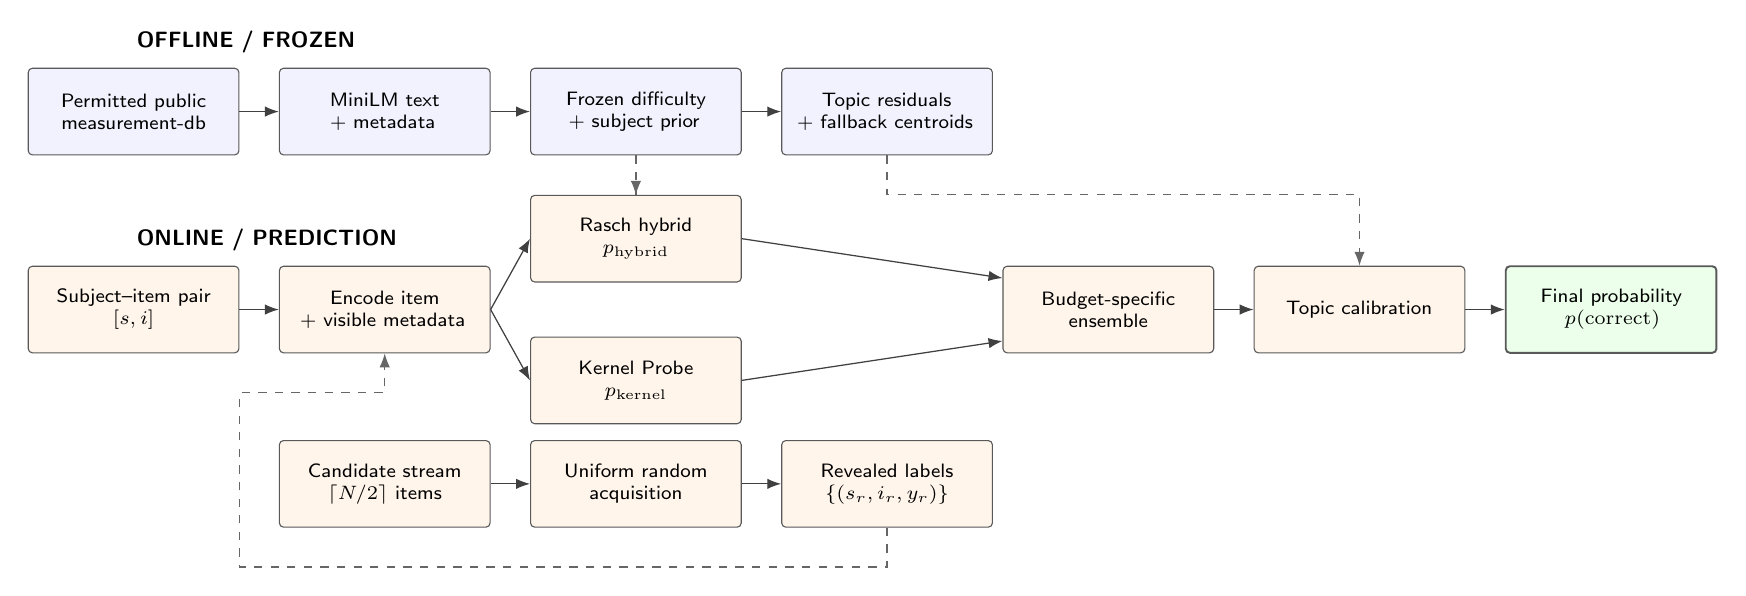
\begin{tikzpicture}[
  >=Latex,
  font=\sffamily\scriptsize,
  node distance=5mm and 5mm,
  box/.style={draw=black!65, rounded corners=1.5pt, align=center,
              text width=25mm, minimum height=11mm, inner sep=2.5pt},
  blendbox/.style={box, minimum height=22mm},
  offline/.style={box, fill=blue!5},
  online/.style={box, fill=orange!8},
  output/.style={box, fill=green!8, line width=.7pt},
  flow/.style={->, line width=.45pt, draw=black!75},
  feedback/.style={->, dashed, line width=.45pt, draw=black!60},
  lane/.style={font=\sffamily\bfseries\footnotesize, inner sep=1pt}
]

% Offline preparation: equal-width nodes on one baseline.
\node[offline] (data) {Permitted public\\measurement-db};
\node[offline, right=of data] (features) {MiniLM text\\+ metadata};
\node[offline, right=of features] (models) {Frozen difficulty\\+ subject prior};
\node[offline, right=of models] (cal) {Topic residuals\\+ fallback centroids};
\draw[flow] (data.east) -- (features.west);
\draw[flow] (features.east) -- (models.west);
\draw[flow] (models.east) -- (cal.west);
\node[lane, above=1.5mm of data, anchor=south west] {OFFLINE / FROZEN};

% Online prediction path. Rasch and kernel are parallel branches.
\node[online, below=14mm of data] (input) {Subject--item pair\\$[s,i]$};
\node[online, right=of input] (encode) {Encode item\\+ visible metadata};
\node[online, right=of encode, yshift=9mm] (rasch) {Rasch hybrid\\$p_{\rm hybrid}$};
\node[online, right=of encode, yshift=-9mm] (kernel) {Kernel Probe\\$p_{\rm kernel}$};
\node[blendbox, online, right=of encode, xshift=60mm] (blend) {Budget-specific\\ensemble};
\node[online, right=of blend] (adjust) {Topic calibration};
\node[output, right=of adjust] (pred) {Final probability\\$p(\mathrm{correct})$};
\draw[flow] (input.east) -- (encode.west);
\draw[flow] (encode.east) -- (rasch.west);
\draw[flow] (encode.east) -- (kernel.west);
\coordinate (blendtop) at ($(blend.west)+(0,4mm)$);
\coordinate (blendbottom) at ($(blend.west)+(0,-4mm)$);
\draw[flow] (rasch.east) -- (blendtop);
\draw[flow] (kernel.east) -- (blendbottom);
\draw[flow] (blend.east) -- (adjust.west);
\draw[flow] (adjust.east) -- (pred.west);
\node[lane, above=1.5mm of input, anchor=south west] {ONLINE / PREDICTION};

% Acquisition/update row. The three boxes share a baseline.
\node[online, below=11mm of encode] (candidates) {Candidate stream\\$\lceil N/2\rceil$ items};
\node[online, right=of candidates] (acq) {Uniform random\\acquisition};
\node[online, right=of acq] (labels) {Revealed labels\\$\{(s_r,i_r,y_r)\}$};
\draw[flow] (candidates.east) -- (acq.west);
\draw[flow] (acq.east) -- (labels.west);

% Feedback follows a dedicated outer route below the acquisition row.
% It enters the online encoder from below, so no dashed segment crosses a box.
\coordinate (feedbackdown) at ($(labels.south)+(0,-5mm)$);
\coordinate (feedbackleft) at ($(candidates.west)+(-5mm,0)$);
\coordinate (feedbackunder) at ($(encode.south)+(0,-5mm)$);
\draw[feedback] (labels.south) -- (feedbackdown) -| (feedbackleft) |- (feedbackunder) -- (encode.south);

% Frozen artifacts enter the corresponding online stages through orthogonal paths.
\draw[feedback] (models.south) -- ++(0,-5mm) -| (rasch.north);
\draw[feedback] (cal.south) -- ++(0,-5mm) -| (adjust.north);
\end{tikzpicture}
}
  \caption{ASRP overview. Frozen public-data artifacts supply difficulty, prior, and calibration estimates. Revealed labels adapt the Rasch hybrid and kernel probe before budget-specific ensembling and topic correction. The source guard is inactive for anonymous proxy identifiers. Candidate pools contain half of each complete group. Random samples uniformly; Adaptive skips up to 16 warm-up candidates before covariance-gain selection. Both supply nested label prefixes.}
  \label{fig:method}
\end{figure}

\subsection{Item representation and amortized difficulty}

Let $e_i\in\mathbb{R}^{384}$ be the sentence embedding of the normalized item text from MiniLM. We concatenate $e_i$ with six deterministic numeric text features $z_i\in\mathbb{R}^{6}$ (including text length, digit proportion, and code or mathematical markers). The \textbf{frozen difficulty network} standardizes this vector and applies a three-layer feed-forward map (390--128--32--1):
\[
  d_i=f_{\phi}([e_i;z_i]).
\]
To compute $e_i$, the whitespace-normalized text is restricted to its first 6,000 characters and tokenized to at most 256 tokens. Mean pooling and $L_2$ normalization yield $e_i$. The hidden layers use ReLU activations; standardized inputs are clipped to $[-10,10]$ and the resulting difficulty to $[-2,2]$. This content-based estimate is an amortized substitute for fitting a separate difficulty parameter for every unseen item.

\subsection{Public prior and Rasch update}

The hybrid uses two public-data priors. The subject-only prior initializes ability, while the metadata prior $p_{\mathrm{src}}$ combines the subject's public response rate with visible item-feature statistics for evidence smoothing. For the frozen public subject offset $o_s$ keyed by normalized model name (zero for an unknown name), define
\[
  m_s=\operatorname{clip}(0.5+0.5o_s,0.05,0.95),\qquad
  \theta_0=\operatorname{logit}(m_s).
\]
The Rasch probability is
\[
  p_{\mathrm{Rasch}}(i)=\sigma(\theta-d_i),
  \quad \sigma(z)=\frac{1}{1+e^{-z}}.
\]
Here $d_i$ is the frozen content-based item difficulty from Section~4.1. For acquired labels $(y_k,d_k)_{k=1}^{n}$, ASRP obtains a \textbf{maximum a posteriori (MAP) estimate} by maximizing the Bernoulli log-likelihood with a Gaussian prior centered at $\theta_0$:
\[
 \ell(\theta)=\sum_{k=1}^{n}\log p(y_k\mid\theta,d_k)
                 -\frac{(\theta-\theta_0)^2}{2v},
 \qquad v=2.0.
\]
The implementation uses Newton--Raphson iteration with clipped steps. Writing $p_k=\sigma(\theta-d_k)$,
\[
 g=\sum_k(y_k-p_k)-\frac{\theta-\theta_0}{v},\qquad
 h=\sum_k p_k(1-p_k)+\frac{1}{v},\qquad
 \theta\leftarrow\theta+\operatorname{clip}(g/h,-2,2).
\]
It stops when the step magnitude is below $10^{-7}$ or after 30 iterations, and clips the final ability to $[-12,12]$. At budget zero, $\theta=\theta_0$.

The metadata prior supplies a smoothed evidence estimate,
\[
 p_{\mathrm{smooth}}=\frac{S_n+\kappa p_{\mathrm{src}}}{n+\kappa},
 \qquad S_n=\sum_k y_k,\quad \kappa=4.
\]
The Rasch and smoothed terms are combined as
\[
 p_{\mathrm{hybrid}}=(1-\lambda_n)p_{\mathrm{smooth}}+\lambda_n p_{\mathrm{Rasch}},
\]
with frozen $\lambda_n=(0.2875,0.3000,0.2875,0.2750,0.2250,0.2375)$ for budgets $(0,1,3,7,15,31)$.

\subsection{Support-conditioned kernel probe}

The \textbf{support-conditioned kernel probe} estimates a local correction from the revealed support items. The support contains revealed responses from the current benchmark, potentially spanning multiple subjects. For each support item $r$, let $u_r$ be its MiniLM vector and $v_r$ its hashed lexical vector, both derived from visible item text, metadata, and interactor descriptions. Unlike the Rasch text encoder, the kernel encoder pools up to four evenly spaced 254-token windows, normalizes each window vector, and normalizes their sum. The lexical vector has 8,192 hashed coordinates. For support size $m>1$, we center and scale the semantic coordinates and apply inverse-frequency weights to lexical coordinates:
\[
 \tilde u_r=\operatorname{norm}((u_r-\bar u)\odot a),\qquad
 \tilde v_r=\operatorname{norm}(v_r\odot b).
\]
Here $\operatorname{norm}$ denotes $L_2$ normalization, $\bar u$ is the support mean, $a$ is an inverse standard-deviation scale regularized by the median support variance (floored at $10^{-7}$), and $b_\ell=\log((1+m)/(1+f_\ell))+0.1$, where $m$ is the support size and $f_\ell$ counts support vectors with a nonzero lexical coordinate $\ell$. For a single support item, centering and coordinate reweighting are bypassed. For two support items, the similarity kernel is
\[
 q_{rt}=\frac{\tilde u_r^\top\tilde u_t+\tilde v_r^\top\tilde v_t}{2},\qquad
 K_{rt}=\exp\!\left(\frac{\min(q_{rt}-1,0)}{\tau}\right),
\]
with $\tau=4\max(d_{\mathrm{med}},10^{-5})$, where $d_{\mathrm{med}}$ is the median off-diagonal distance $1-q_{rt}$ above $10^{-8}$, or $0.1$ if none qualifies. The query-to-support vector $k(x)$ uses the same transformation and kernel.

The kernel intercept is a two-component Beta mixture. For subject $a$, let $s_a$ of $n_a$ revealed labels be successes and let $o_a$ be the public offset. Define $m_a=\operatorname{clip}(0.5+0.5o_a,0.05,0.95)$. For concentrations $c\in\{1,8\}$ and prior masses $\pi_1=0.3$, $\pi_8=0.7$,
\[
 \alpha_{ac}=m_ac,\quad \beta_{ac}=(1-m_a)c,\quad
 \omega_{ac}\propto\pi_c\frac{\mathrm{B}(\alpha_{ac}+s_a,\beta_{ac}+n_a-s_a)}
 {\mathrm{B}(\alpha_{ac},\beta_{ac})},
\]
\[
 b_a=\sum_c\omega_{ac}\frac{\alpha_{ac}+s_a}{c+n_a}.
\]
Here $\mathrm{B}$ is the beta function and the posterior weights are normalized so that $\sum_c\omega_{ac}=1$. Thus $b_a$ is the conservative subject baseline before using local similarity.

Let $M$ average rows belonging to the same subject, and let $C=I-M$. The centered ridge residual coefficients are
\[
 \gamma=C(CKC+\lambda I)^{-1}Cy,\qquad \lambda=0.3,
\]
where $y$ contains the revealed binary labels. If $\bar f_a$ is the subject mean of the fitted kernel contribution, the query prediction is
\[
 p_{\mathrm{kernel}}(x,a)=\operatorname{clip}\!\left(b_a+k(x)^\top\gamma-\bar f_a,0,1\right).
\]
The kernel contribution is suppressed at budgets 0 and 1 and receives weights $(0,0,0.2,0.4,1,1)$ at $(0,1,3,7,15,31)$, so a tiny support set cannot override the cold-start prediction. This creates a deliberate budget-dependent division of labor: at low budgets, the Rasch hybrid is the main predictor because its public subject prior and content-based difficulty remain stable when there are too few revealed labels to fit a local kernel residual. The kernel branch is introduced gradually at 3 and 7 labels, then becomes the nominal primary predictor at 15 and 31 labels, giving greater influence to residual corrections fitted from the larger support set. The late-budget source guard can reduce this kernel weight for sources with a regression identified in public diagnostics.

\subsection{Topic calibration and source guard}

The calibration artifact is generated from public binary responses. ASRP scans the visible metadata in its original order and uses the first topic key--value pair present in the frozen topic-residual table. A topic residual $r_{t,n}$ is shrunk toward zero using its public count $m_t$:
\[
  \Delta_{t,n}=\operatorname{clip}\!\left(
    \frac{m_t}{m_t+40}r_{t,n},-0.06,0.06\right).
\]
If no topic key--value pair matches the table, the Rasch encoder's 384-dimensional vector is assigned to the closest of eight frozen centroids by cosine similarity. Cluster residuals use a stronger prior count of 200 and a smaller cap of $0.03$. The correction is applied after the budget-specific ensemble.

Public validation identified some sources for which the kernel branch became less accurate at high budgets. At budgets 15 and 31, a matching public-source key supplies a guard $g\in[0,0.35]$ that multiplies the nominal kernel weight by $1-g$; the remaining weight goes to the Rasch hybrid. Unmatched identifiers receive zero adjustment. The anonymous aliases in the reproducible proxy do not match these source-name keys, so this guard is inactive in the reported experiment. This guard is a conservative regularizer, not a lookup of hidden test outcomes; source statistics are learned offline from public data.

\subsection{Adaptive acquisition}

The submitted \textbf{\texttt{labeling.py}} implements \textbf{\texttt{adaptive\_4\_warm}}. The policy can skip up to 16 early candidates to establish a local feature geometry, subject to the evaluator's remaining-item constraint. It then estimates the conditional covariance reduction from each candidate using previously revealed items, previously seen candidate features, the current candidate, and the supplied context. The candidate's gain ratio is raised to power four and converted to a probability under the remaining label budget. When the number of remaining candidates equals the remaining label budget, the hook acquires every remaining candidate. The hook never accesses future candidates or evaluation outcomes.

\section{Experimental setup}

\subsection{Public proxy protocol}

\paragraph{Complete groups and repeated splits.}
Eligible groups contain 80--1,000 distinct items before splitting. Within each eligible source, SHA256 ordering with the fixed group-selection seed 20261028 selects one subject, identically across all experiments. The actual group sizes range from \ProxyMinItems{} to \ProxyMaxItems{}. For repeated responses to an item, the smallest trial number and then response ID select one binary outcome, held fixed across policies and seeds. Splitting uses seeds \textbf{42, 43, and 44}: a seeded SHA256 ordering assigns the first $\lceil N/2\rceil$ items to acquisition and the rest to evaluation. Thus candidate pools contain \ProxyMinPool{}--\ProxyMaxPool{} items, and each seed scores \textbf{\ProxyTargets{} evaluation outcomes}. The dataset revision, table checksums, subject IDs, response IDs, and three splits are fixed in the released manifest.

\paragraph{Paired predictor and acquisition comparison.}
We evaluate \textbf{ASRP and Empirical Mean under both Random and Adaptive acquisition}. Within a seed, both policies see the same candidate order and evaluation pool. Random acquisition accepts the current candidate with probability $L/R$, where $L$ is the remaining label budget and $R$ counts remaining candidates including the current one. Its random variates are deterministic hashes of the visible input and context, with seed-specific anonymous subject aliases. Adaptive acquisition executes the packaged \texttt{adaptive\_4\_warm} hook. Its warm-up is $\min(16,A-31)$ for a candidate pool of size $A$; remaining candidates are mandatory when their count equals the remaining budget. Both predictors receive identical acquired labels \emph{within each policy}, using nested prefixes at budgets $0,1,3,7,15,31$. The two policies can select different labels. Every checkpoint scores the same evaluation items within that seed.

\paragraph{Scope and selection capacity.}
We additionally report the prespecified subset of \ProxyLargeGroups{} groups with at least 160 items, hence at least 80 candidates, to examine acquisition where the pool leaves more room for selection after warm-up. Small eligible groups remain in the primary results. Evaluation outcomes are never supplied online, but this acquisition/evaluation split is not independent of all offline fitting: frozen public training and calibration use the same release. The local scores may therefore be optimistic. They are not Codabench scores; private data and formative random draws can produce different results.

\subsection{Baseline and metrics}

We use the \textbf{Empirical Mean predictor} from the official PAIEC repository \citep{paiec_baselines}. For $n$ acquired binary labels in the current subject--benchmark group, it predicts
\[
 p_{\mathrm{EM}}=
 \begin{cases}
  0.5, & n=0,\\
  \frac{1}{n}\sum_{k=1}^{n}y_k, & n>0.
 \end{cases}
\]
It uses neither item features nor a learned prior. We run this unchanged predictor on each policy's acquired evidence. Empirical Mean + Random corresponds to its default acquisition choice; Empirical Mean + Adaptive isolates the effect of giving the same predictor ASRP's selected labels. The local Random policy reproduces uniform sampling without replacement, not the private server's particular random draw.

For each seed and policy, we compute Brier scores within each subject--source group and average groups equally, then average the three seed-level scores equally. Groups have different numbers of evaluation items, so pooling all response rows would give different weights and is not used. Brier ALC uses the weights in Section~2. We report the individual seed ALCs and their sample standard deviation; these describe variation across the three specified splits, not a confidence interval over all possible evaluations.

\section{Results and analysis}

\subsection{Public proxy results}

Across 30 fixed public-data draws, \textbf{ASRP + Adaptive reaches mean Brier ALC $0.1907$}, compared with $0.2294$ for Empirical Mean using the same labels (Table~\ref{tab:proxy}). Each draw contains complete groups under the 1,000-pair cap; Table~\ref{tab:seeds} reports variation across these changing group compositions.


\begin{table}[H]
\centering
\small
\setlength{\tabcolsep}{4pt}
\begin{tabular}{lrrrrrrr}
\toprule
Predictor + acquisition & $B_0$ & $B_1$ & $B_3$ & $B_7$ & $B_{15}$ & $B_{31}$ & ALC\\
\midrule
Empirical Mean + Random & 0.2500 & 0.3488 & 0.2518 & 0.2086 & 0.1910 & 0.1842 & 0.2435\\
Empirical Mean + Adaptive & 0.2500 & 0.3594 & 0.2366 & 0.2003 & 0.1883 & 0.1837 & 0.2403\\
ASRP + Random & 0.2277 & 0.2165 & 0.2069 & 0.1945 & 0.1845 & 0.1755 & 0.2008\\
ASRP + Adaptive & 0.2277 & 0.2154 & 0.2035 & 0.1912 & 0.1819 & 0.1738 & 0.1985\\
\bottomrule
\end{tabular}

\vspace{6pt}
\caption{Public proxy Brier scores averaged equally over \ProxySources{} groups and seeds 42, 43, and 44. Lower is better. Evaluation pools are matched across policies; acquired labels are matched across predictors within each policy.}
\label{tab:proxy}
\end{table}

\begin{figure}[H]
  \centering
  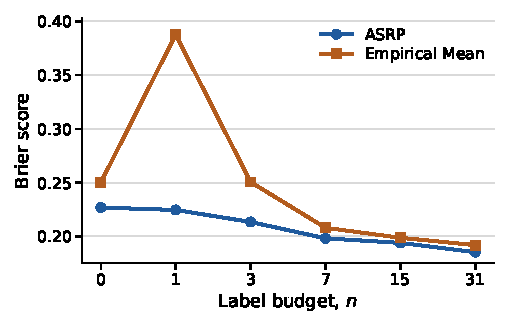
\includegraphics[width=0.95\columnwidth,height=0.24\textheight,keepaspectratio]{figures/public_proxy_curve.pdf}
  \caption{Mean public-proxy Brier curves for the four predictor--acquisition combinations on the official $\log_2(1+n)$ budget axis. Solid lines denote Adaptive acquisition and dashed lines Random; values match Table~\ref{tab:proxy}.}
  \label{fig:proxy_curve}
\end{figure}

\begin{table}[H]
\centering
\small
\begin{tabular}{lrrrr}
\toprule
Predictor (Random acquisition) & Mean ALC & SD & Minimum & Maximum\\
\midrule
Empirical Mean & 0.2285 & 0.0701 & 0.0286 & 0.3613\\
ASRP & 0.1895 & 0.0533 & 0.0260 & 0.2549\\
\bottomrule
\end{tabular}

\vspace{6pt}
\caption{Group-averaged Brier ALC for each split/acquisition seed. SD is the sample standard deviation over the three seed scores. Lower ALC is better.}
\label{tab:seeds}
\end{table}

\subsection{Prediction and acquisition effects}

\paragraph{Matched-evidence comparison.} With randomly acquired evidence held fixed, ASRP changes ALC by $-0.0391$ relative to Empirical Mean and scores lower in 28 of 30 draws. The comparison measures the complete predictor under the same label-selection rule. Draw-level SD describes variability in the sampled public group compositions.


\section{Limitations}

\paragraph{Sparse metadata and local adaptation.}
Some public items lack usable topic metadata, motivating the frozen embedding-cluster fallback. Topic groups with few observations can have residual estimates dominated by sampling noise. This motivates shrinking and capping topic corrections. Likewise, an unrepresentative acquired support set can cause the kernel to over-update. The source guard only limits its weight when a public-source key matches; anonymous or unseen sources do not receive this adjustment. These considerations motivate conservative correction magnitudes; neither topic calibration nor local adaptation guarantees improvement on every source.

\section{Reproducibility and disclosure}

The release separates inference code in \path{src/asrp} from frozen artifacts in \path{artifacts/asrp}. The entry points are \texttt{model.py} and \texttt{labeling.py}. From the repository root, run:

\begin{verbatim}
uv sync --locked
uv run hf auth login
uv run --locked python tools/reproduce.py
\end{verbatim}

After accepting upstream access conditions and authenticating with a Hugging Face read token, this command downloads and verifies the pinned tables, reconstructs all splits, builds the submission, and evaluates all four combinations at three seeds. It checks every prediction against the published run within $10^{-7}$ and requires identical acquired labels. Frozen weights are used directly without refitting or parameter selection.

\path{experiments/} records the protocol, checksums, and selected subject/item/response IDs. \path{results/proxy} contains predictions, acquired labels, decisions, and metrics. \path{tools/update_report_results.py} generates the reported numbers; task text is downloaded from upstream.

Kernel weights are in \path{src/asrp/model.py}; Rasch settings and calibration are in \path{artifacts/asrp/runtime_config.json} and \path{artifacts/asrp/topic_calibration.json}. Code, frozen weights, the locked CPU environment, and report source are available at \url{https://github.com/Hubert0916/arsp}. The official checker remains in the upstream starting kit.

The competition-specific artifacts were produced from the permitted public measurement-db inventory. We use the pretrained MiniLM encoder and cite its model family. Codex was used as a coding assistant during development; it is not used as an online predictor in the current submission. No API key is included in the codebase or report.

\section{Conclusion}

ASRP provides a practical, budget-aware predictor for subject--item capability evaluation. Its main engineering principle is to use content-based and psychometric structure at cold start, use support-conditioned residuals only when evidence is available, and shrink topic corrections and late-budget updates toward conservative defaults. The three-seed public proxy gives ASRP + Adaptive a mean Brier ALC of $0.1987$. Compared with Random acquisition using the same predictor, Adaptive reduces mean ALC by $0.0021$. The paired design separates changes in prediction quality from changes in which labels are acquired.


\appendix
\section{Public source inventory}\label{app:sources}

The following \ProxySources{} public binary source identifiers occur in the paired three-seed evaluation. They identify the evaluation sources; the benchmark inventory and upstream licenses remain authoritative.

\begingroup
\scriptsize
\begin{verbatim}
afrieval
agentic_review_perturbation
algotune
alignment_faking
appworld
averimatec
babilong
beavertails
benger
bird_sql
braveguard
bridging_gap
cellverse
critic_discernment_game
crow
devbench
editbench
edu_circuit_hw
egoschema
elicitation_game
engdesign
enginemt_qa
exploitgym
faithcot
fewshot_ttt_bbh
financebench
finegrain_t2i
hallusionbench
harmbench
healthadminbench
helm_bbq
helm_thaiexam
hle
igakuqa119
ikp
jailbreakbench
kernelbench
legal_rag_bench
llmail_inject
llms_lean_formalization
mathconstraint
mathvista_mini
medhelm_ehr_sql
medhelm_head_qa
medhelm_med_mcqa
medhelm_med_qa
medhelm_medbullets
medhelm_medcalc_bench
medhelm_medec
medhelm_medhallu
medhelm_pubmed_qa
medhelm_race_based_med
mj_bench
mmbench_v11
monkey_power_laws
morphkv
mtbbench
multi_swebench
naep_llm_students
naturebench
nester
nyu_ctf_bench
openbiorq
os_harm
perfcodebench
planbench
proofaug
pxplore
real_webagents
realtimeqa
reliancescope
researchcodebench
revolve
risebench
robust_reasoning_benchmark
safeagentbench
sib200
software_world_models
sustainable_food
swe_smith
swebench_live
swepolybench
tau2_bench
taubench
truthfulqa_mc
tulu_human_eval
tumlu
visual_riddles
visualwebarena
vl_rewardbench
workarena
workbench_revisited
\end{verbatim}

\endgroup

% unsrtnat preserves the order in which references first appear in the text.
\bibliographystyle{unsrtnat}
\bibliography{references}


\end{document}
